\section{Introduction. Neutrinos as Fundamental Standard Model Particles}

The Standard Model can be summarized in a table like one at Fig. \ref{fig:StandardModel}. It includes three charged leptons, three neutrinos and six quarks and their antiparticles which are split into three generations. In addition, it includes gauge bosons, Higgs boson and three fundamental interactions: electromagnetic, strong and weak. Charged particles, which include three leptons (electrons, muons and $\tau$-leptons), all quarks, W bosons and their antiparticles can interact electromagnetically, through exchange of virtual photon. Quarks have non-integer electric charges (in units of absolute value of the electron charge) of +2/3 or -1/3. They also possess additional quantum number which is called "color" and can participate in strong couplings, through exchange of gluons. Individual quarks do not exist in the nature, they present in combinations of three quarks or quark-antiquark pairs. Particles composed of three quarks are baryons, and particles composed of quark and antiquark are mesons. Baryons and mesons are always neutral in color, and possess integer electric charge. All baryons and mesons are called hadrons.\\  

All those particles and also neutrinos can interact through weak interactions through charged current (CC), by exchanging W boson, and through neutral current (NC), by exchanging Z boson. The corresponding Feynman diagrams for the NC and CC are shown at Fig. \ref{fig:NuScattering}. Left Feynman diagram shows electron scattering off neutrino through the NC. Any neutrino or antineutrino can scatter off electron with the NC. Moreover, any weakly interacting particle can scatter off any other weakly interacting particle through the NC because $Z^0$ does not transform a particle to any other particle but is just emitted from the fermion line. Middle Feynman diagram at Fig. \ref{fig:NuScattering} shows $e^- \nu_e \rightarrow e^- \nu_e$ scattering through the CC. W boson transforms neutrino into corresponding charged lepton or vice-verse and therefore only $f^- \nu_f \rightarrow f^- \nu_f$ scattering is possible with the CC where $f$ is $e$, $\mu$ or $\tau$. For example, $e^- \nu_\mu \rightarrow e^- \nu_\mu$ scattering is possible through the NC only. Right Feynman diagram shows process of $e^- \bar{\nu_e}$ annihilation with further production of $e^- \bar{\nu_e}$. In principle, any $f^- \bar{\nu_f}$ or $f^+ \nu_f$ pair could get produced by the W boson.\\

\begin{figure}
\caption{Fundamental particles and their interactions according to the Standard Model. There exist three generations of fermions. Fermions interact through the exchange of Gauge Bosons. Charged leptons and quarks (fermions) are subject to electromagnetic interactions (through photons). Quarks also interact strongly (through gluons). All leptons and quarks interact weakly (through $W^{\pm}$ and $Z^0$ bosons). All the fundamental particles of the Standard Model have been discovered, and nothing more. Source of picture: \cite{ref_fig_StandardModel}}
\label{fig:StandardModel}
\centering 
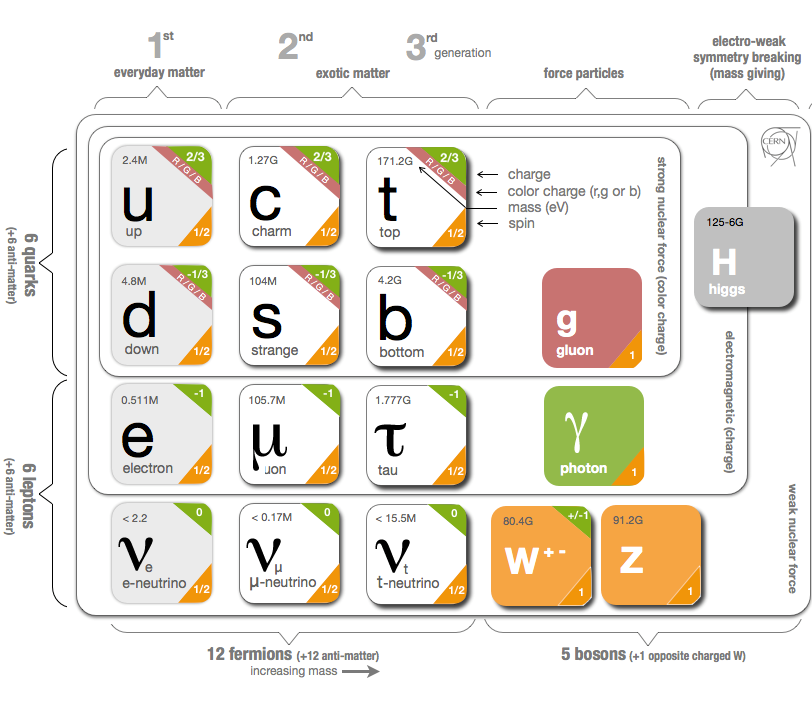
\includegraphics[width=0.83\textwidth, keepaspectratio=true]{figs/StandardModel.png}
\end{figure}

\begin{figure}
\caption{Feynman diagrams of neutral current (NC, left), and charged current (CC, middle and right) neutrino scattering.}
\label{fig:NuScattering}
\centering
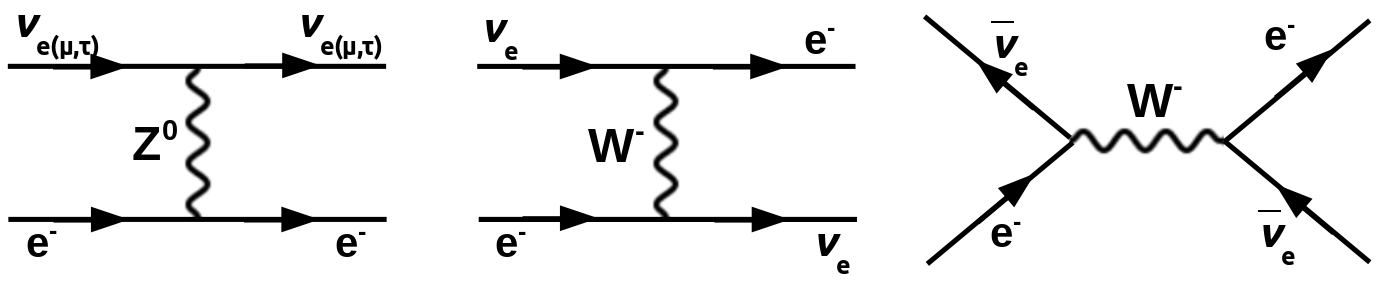
\includegraphics[width=0.80\textwidth, keepaspectratio=true]{figs/neutrinoScattering.png}
\end{figure}


All known substances in the known Universe consist of millions of different species of molecules which are composed by hundreds different species of atoms. Each atom consists of certain number of protons, neutrons and electrons. All protons and neutrons are composed of three quarks (uud for proton and udd for neutron) which are glued together by strong interactions. Therefore, all known substance consists of only three fundamental particles from the Fig. \ref{fig:StandardModel}: u- and d-quarks and electrons. Despite that neutrinos are not part of substances, a large number of them exist in the nature without any human-built machines. Quoting \cite{ref_Griffiths}, 11.1: "John Bahcall, who was responsible for most of the calculations of solar neutrino abundances, liked to say that 100 billion neutrinos pass through your thumbnail every second; and yet they are so ethereal that you can look forward to only one or two neutrino-induced reaction in your body during your entire lifetime".\\

Two very common and well known interactions with neutrino participation are neutron beta decay and muon decay. The Feynman diagrams of these processes are shown in Fig. \ref{fig:MuonAndNeutronDecays}. The mean lifetime of a free neutron is $~15$ minutes and it decays by $n \rightarrow p + e^- + \bar{{\nu}_e} $ \cite{ref_PDG}. At the level of fundamental particles, neutrons consist of two d-quarks and one u-quark and in the beta decay one of the d-quarks transforms into a u-quark through the weak interaction mediated by a $W^- $ boson. Thus, the proton, which consists of two u-quarks and one d-quark, is being produced from the neutron decay. When this happens, the electron and electron antineutrino are emitted to conserve the charge and the lepton flavor number. Examples of the neutron beta decay in nature include ${^{49}}{_{19}}K \rightarrow {^{40}}{_{20}}Ca$, ${^{64}}{_{29}}Cu \rightarrow {^{64}}{_{30}}Zn$, ${^3}{_1}H \rightarrow {^3}{_2}He$ \cite{ref_Griffiths} (the positive beta decay,  $p \rightarrow n + e^+ + {\nu}_e $, is forbidden for free proton by energy conservation but it is allowed in certain cases when a proton is part of a nuclei). Such reactions are widely used for neutrino and antineutrino detection.\\

As for a muon, it's mean lifetime is $~2 {\mu}s$, and it decays as ${\mu}^- \rightarrow e^- + {\nu}_{\mu} + \bar{{\nu}_e}$ through the W boson. This process is also common in nature, in cosmic rays as shown at Fig. \ref{fig:cosmicMuons}. Highly energetic cosmic protons scatter off the atmosphere molecules, for instance, as $p+p \rightarrow n+p+\pi^+$, $p+n \rightarrow n+n+\pi^-$, $p+p \rightarrow p+p+\pi^0$. Several additional hadrons can be produced in the reaction. If $\pi^0$ is produced, it decays to two photons $\pi^0 \rightarrow \gamma\gamma$. Charged pions decay $\pi^{\pm} \rightarrow \mu^{\pm} + \nu_\mu(\bar{\nu_\mu})$ and then some number of muons decay $\mu^{\pm} \rightarrow e^{\pm} + \nu_e(\bar{\nu_e}) + \bar{\nu_\mu}(\nu_\mu)$ while traveling through the atmosphere to the ground. Feynman diagram of muon decay is shown at Fig. \ref{fig:MuonAndNeutronDecays}. Muon transforms to muon neutrino with emission of W boson, than W boson decay to electron and electron antineutrino.\\

\begin{figure}
\caption{Feynman diagrams of (left) neutron and (right) muon decays. Neutron beta decay is a d-quark transforming into u-quark through the W boson emission of an electron and an electron antineutrino. A muon decays into an electron, a muon neutrino and an electron antineutrino through a W boson}
\label{fig:MuonAndNeutronDecays}
\centering
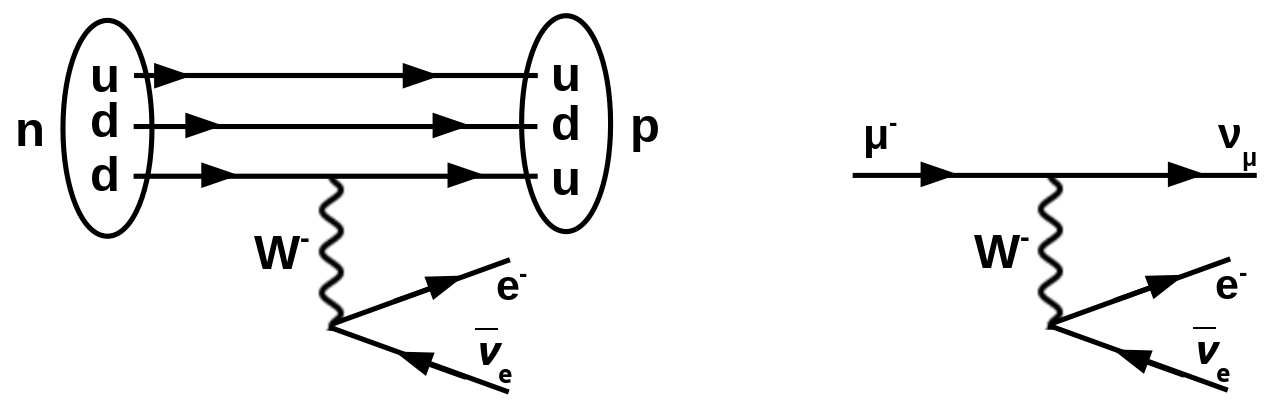
\includegraphics[width=0.70\textwidth, keepaspectratio=true]{figs/NeutronAndMuonDecays.png}
\end{figure}

\begin{figure}
\caption{Cosmic shower induced by scattering of the incident cosmic proton off an air molecule. Charged and neutron pions are born in the reaction and then they further decay as $\pi^0 \rightarrow \gamma\gamma$, $\pi^+ \rightarrow \mu^+ + \nu_\mu$, $\pi^- \rightarrow \mu^- + \bar{\nu_\mu}$.}
\label{fig:cosmicMuons}
\centering
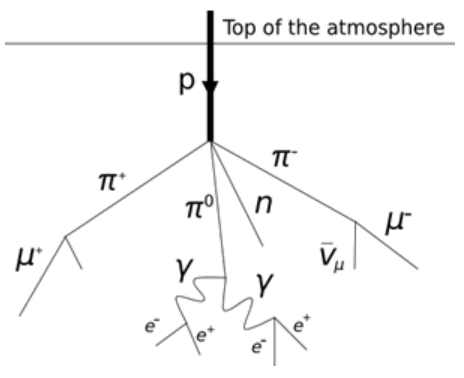
\includegraphics[width=0.60\textwidth, keepaspectratio=true]{figs/cosmicMuons.png}
\end{figure}



There are three flavors of neutrinos, one for each generation: electron neutrino, muon neutrino, and $\tau$-neutrino. In the processes described above (neutron beta decay and muon decay) the lepton flavor numbers $L_e$, $L_{\mu}$ and $L_{\tau}$ are conserved. The table \ref{tab:LeptonFlavorNumber} shows the value of this number for all leptons and anti-leptons. \\

\begin{table}[h]
  \begin{center}
  \caption{ Lepton Flavor Number}
  \begin{tabular}{|c|c|c|c|}
     particles & $L_e$ & $L_{\mu}$ & $L_{\tau}$ \\ \hline
     $e^-,\nu_e$ &  +1  &  0  &  0  \\ \hline 
     $e^+, \bar{\nu_e}$ &  -1  &  0  &  0  \\ \hline 
     $\mu^-,\nu_{\mu}$ &  0  &  +1  &  0  \\ \hline 
     $\mu^+, \bar{\nu_{\mu}}$ &  0  &  -1  &  0  \\ \hline 
     $\tau^-,\nu_{\tau}$ &  0  &  0  &  +1  \\ \hline 
     $\tau^+, \bar{\nu_{\tau}}$ &  0  &  0  &  -1  \\ \hline 
  \end{tabular}
  \label{tab:LeptonFlavorNumber}
  \end{center}
\end{table}

Lepton flavor numbers are conserved in almost all particle physics processes and the only violation of this law ever observed is through neutrino oscillations: the ability of a neutrino to change flavor.\\

This paper is about neutrino oscillations. Chapter 2 of this paper reviews the theoretical background of the neutrino oscillations starting from a simplified two-neutrino model in vacuum to a three-neutrino model in presence of matter and also discusses possible mechanisms to give neutrinos mass. Chapter 3 gives a historical background of related experimental measurements including the first evidence of neutrino oscillations, milestones achieved by the scientific community in measuring different neutrino oscillation parameters including the most recent experimental results. Chapter 4 explains the need of the new experiment and gives an overview of the proposed LBNF/DUNE experiment in terms of its physics program and experimental setup. It also discusses the advantages of LBNF/DUNE by comparison of the other experiments of this kind. Chapter 5 draws conclusions on the potential scientific impact of the proposed LBNF/DUNE project.  


